\lab{The Finite Difference Method}{The Finite Difference Method}
\label{lab:finitedifference2}

\objective{The finite difference method provides a solid foundation for solving partial differential equations.
Understanding and applying finite difference is key to understanding numerical solutions to PDEs.}
\labdependencies{NumericalIVP}

A \textbf{finite difference} for a function $f(x)$ is an expression of the form $f(x+s)-f(x+t)$.
Finite differences can give a good approximation of derivatives.

Suppose we have a function $u(x)$, defined on an interval $[a,b]$.
Let $a = x_0, x_1, \ldots x_{n-1}, x_n=b$ be a grid of $n+1$ evenly spaced points, with $x_{i+1}-x_i = h$, where $h = (b-a)/n$.

You are used to seeing the derivative $u'(x)$, which can written in centered-difference form as:
\begin{align*}
u'(x)=\lim_{h\to\infty}\frac{u(x+h)-u(x-h)}{2h}.
 \end{align*}
Suppose we are interested in knowing the value of the derivative at the points $\{x_i\}$.
Even if we don't have a formula for $u'(x)$, we can approximate it using finite differences.
We first write the Taylor polynomial expansion of $u(x+h)$ and $u(x-h)$ centered at $x$.
This gives
\begin{align}
u(x+h)=u(x)+u'(x)h+\frac{1}{2}u''(x)h^2+\frac{1}{6}u'''(x)h^3+\mathcal{O}(h^4)\label{plus}\\
u(x-h)=u(x)-u'(x)h+\frac{1}{2}u''(x)h^2-\frac{1}{6}u'''(x)h^3+\mathcal{O}(h^4)\label{minus}
\end{align}
Subtracting \eqref{minus} from \eqref{plus} and rearranging gives
\begin{align*}
u'(x)=\frac{u(x+h)-u(x-h)}{2h}+\mathcal{O}(h^2).
\end{align*}

In terms of our grid points $\{x_i\}$, we have:
\begin{align*}
u'(x_i) \approx \frac{u(x_i+h)-u(x_i-h)}{2h}=\frac{u(x_{i+1})-u(x_{i-1})}{2h}.
\end{align*}
We won't worry about the derivative at the endpoints, $u'(x_0)$ and $u'(x_n)$.
This allows us to approximate the values $\{u'(x_i)\}$ as the solution to a system of equations:
\begin{align}
\frac{1}{2h}
\begin{array}{c}
\begin{bmatrix}
-1 &0 & 1 & \\
& -1 & 0 & 1  \\
& & \ddots & \ddots & \ddots & \\
& & & -1 & 0 & 1 \\
& & & & -1 & 0 & 1
\end{bmatrix}\\
{\scriptstyle\textcolor{red}{(n-1)\times(n+1)}}
\end{array}\cdot
\begin{array}{c}
\begin{bmatrix}
u(x_0) \\ u(x_1)\\ \vdots  \\ u(x_{n-1}) \\ u(x_n)
\end{bmatrix}\\
{\scriptstyle\textcolor{red}{(n+1)\times1}}
\end{array} \approx
\begin{array}{c}
\begin{bmatrix}
u'(x_1) \\ u'(x_2)\\ \vdots  \\ u'(x_{n-2}) \\ u'(x_{n-1})
\end{bmatrix}\\
{\scriptstyle\textcolor{red}{(n-1)\times1}}
\end{array}.
\label{finitedifference2:up}
\end{align}

\noindent This can be rewritten with a $(n-1)\times(n-1)$ tridiagonal matrix instead:
\begin{align}
\frac{1}{2h}
\begin{array}{c}
\begin{bmatrix}
0 & 1 & \\
-1 & 0 & 1  \\
& \ddots & \ddots & \ddots \\
& & -1 & 0 & 1 \\
& & & -1 & 0
\end{bmatrix}\\
{\scriptstyle\textcolor{red}{(n-1)\times(n-1)}}
\end{array}\cdot
\begin{array}{c}
\begin{bmatrix}
u(x_1) \\ u(x_2)\\ \vdots  \\ u(x_{n-2}) \\ u(x_{n-1})
\end{bmatrix}\\
{\scriptstyle\textcolor{red}{(n-1)\times1}}
\end{array} +
\begin{array}{c}
\begin{bmatrix}
-u(x_0)/(2h) \\ 0 \\ \vdots  \\ 0 \\ u(x_n)/(2h)
\end{bmatrix}\\
{\scriptstyle\textcolor{red}{(n-1)\times1}}
\end{array} \approx
\begin{array}{c}
\begin{bmatrix}
u'(x_1) \\ u'(x_2)\\ \vdots  \\ u'(x_{n-2}) \\ u'(x_{n-1})
\end{bmatrix}\\
{\scriptstyle\textcolor{red}{(n-1)\times1}}
\end{array}.
\label{finitedifference2:u}
\end{align}

\noindent Next, we will consider the approximation for $u''(x)$.
If we let
\[u'(x) \approx \frac{u(x+\frac{h}{2})-u(x-\frac{h}{2})}{h}\]
then
\[u''(x) \approx \frac{u'(x+\frac{h}{2})-u'(x-\frac{h}{2})}{h} \approx \frac{\frac{u((x+\frac{h}{2})+\frac{h}{2})-u((x+\frac{h}{2})-\frac{h}{2})}{h}-\frac{u((x-\frac{h}{2})+\frac{h}{2})-u((x-\frac{h}{2})-\frac{h}{2})}{h}}{h}\]
\[= \frac{u(x+h) - 2u(x) + u(x-h)}{h^2}\]
You can achieve the same result by again consider the Taylor polynomial expansion and adding \eqref{plus} and \eqref{minus} and rearranging.
Thus
\[u''(x_i) \approx \frac{u(x_i+h) - 2u(x_i) + u(x_i-h)}{h^2}= \frac{u(x_{i+1}) - 2u(x_i) + u(x_{i-1})}{h^2}\]
Again ignoring the second derivative at the endpoints, this can be written in matrix form as
\begin{align}
\frac{1}{h^2}
\begin{array}{c}
\begin{bmatrix}
1 & -2 & 1 & \\
& 1 & -2 & 1  \\
& &\ddots &\ddots & \ddots  \\
& & & 1 & -2 & 1 \\
& & & & 1 & -2 & 1
\end{bmatrix}\\
{\scriptstyle\textcolor{red}{(n-1)\times(n+1)}}
\end{array}\cdot
\begin{array}{c}
\begin{bmatrix}
u(x_0) \\ u(x_1)\\ \vdots  \\ u(x_{n-1}) \\ u(x_n)
\end{bmatrix}\\
{\scriptstyle\textcolor{red}{(n+1)\times1}}
\end{array}
 \approx
 \begin{array}{c}
\begin{bmatrix}
u''(x_1) \\ u''(x_2)\\ \vdots  \\ u''(x_{n-2}) \\ u''(x_{n-1})
\end{bmatrix}\\
{\scriptstyle\textcolor{red}{(n-1)\times1}}
\label{finitedifference2:uppp}
\end{array}.
\end{align}
This can also be written with a $(n-1)\times(n-1)$ tridiagonal matrix:
\begin{align}
\frac{1}{h^2}
\begin{array}{c}
\begin{bmatrix}
-2 & 1 & \\
1 & -2 & 1  \\
& \ddots & \ddots & \ddots \\
& & 1 & -2 & 1 \\
& & & 1 & -2
\end{bmatrix}\\
{\scriptstyle\textcolor{red}{(n-1)\times(n-1)}}
\end{array}\cdot
\begin{array}{c}
\begin{bmatrix}
u(x_1) \\ u(x_2)\\ \vdots  \\ u(x_{n-2}) \\ u(x_{n-1})
\end{bmatrix}\\
{\scriptstyle\textcolor{red}{(n-1)\times1}}
\end{array} +
\begin{array}{c}
\begin{bmatrix}
u(x_0)/h^2 \\ 0 \\ \vdots  \\ 0 \\ u(x_n)/h^2
\end{bmatrix}\\
{\scriptstyle\textcolor{red}{(n-1)\times1}}
 \end{array} =
 \begin{array}{c}
\begin{bmatrix}
u''(x_1) \\ u''(x_2)\\ \vdots  \\ u''(x_{n-2}) \\ u''(x_{n-1})
\end{bmatrix}\\
{\scriptstyle\textcolor{red}{(n-1)\times1}}
\label{finitedifference2:upp}
\end{array}
\end{align}

Each of these matrices consists mostly of zeros; that is, they are \textit{sparse}.
So make sure to use \li{scipy.sparse} when constructing these matrices and those that follow in this lab.\footnote{See the Volume 1 lab ``Linear Systems'' for a refresher on sparse matrices.}

\begin{problem}
	Let $u(x) = \sin((x+\pi)^2-1)$.
	Use \eqref{finitedifference2:up} - \eqref{finitedifference2:upp} to approximate $\frac{1}{2}u'' - u'$ at the grid points where $a=0$, $b=1$, and $n=10$.
	Graph the result.
    
    Hint: You may find \li{scipy.sparse.diags} useful.
\end{problem}

The previous equations are not only useful for approximating derivatives, but they can be also used to solve differential equations.
Suppose that instead of knowing the function $u(x)$, we know that $\frac{1}{2}u'' - u' = f$, where the function $f(x)$ is given.
How do we solve for $u(x)$?

\section*{Finite Difference Methods}

Numerical methods for differential equations seek to approximate the exact solution $u(x)$ at some finite collection of points in the domain of the problem.
Instead of analytically solving the original differential equation, defined over an infinite-dimensional function space, they use a well-chosen finite system of algebraic equations to approximate the original problem.

Consider the following differential equation:
\begin{align}
	\begin{split}
	&{ } \epsilon u''(x)-u(x)'= f(x), \quad x \in (0,1), \\
	&{ } u(0) = \alpha, \quad u(1) = \beta.
	\end{split} \label{eqn:singular_perturbed_BVP}
\end{align}
Equation \eqref{eqn:singular_perturbed_BVP} can be written $D u = f,$ where $D = \epsilon \frac{d^2}{dx^2} - \frac{d}{dx}$ is a differential operator defined on the infinite-dimensional space of functions that are twice continuously differentiable on $[0,1]$ and satisfy $u(0) = \alpha$, $u(1) = \beta$.

We look for an approximate solution $\{U_i\}$, where \[U_i \approx u(x_i)\] on an evenly spaced grid of points, $a = x_0, x_1, \ldots, x_n = b$,.
Our finite difference method will replace the differential operator $D = \epsilon \frac{d^2}{dx^2} - \frac{d}{dx}$, (which is defined on an infinite-dimensional space), with finite difference operators (defined on a finite dimensional space).
To do this, we replace derivative terms in the differential equation with appropriate difference expressions.

Recalling that
\begin{align*}
\frac{d^2}{dx^2} u(x_i) &= \frac{u(x_{i+1})- 2u(x_i) + u(x_{i-1})}{h^2} + \mathcal{O}(h^2),\\
\frac{d}{dx} u(x_i) &= \frac{u(x_{i+1})-u(x_{i-1})}{2h} + \mathcal{O}(h^2).
\end{align*}
we define the finite difference operator $D_h$ by
\begin{align}
D_h U_i = \epsilon \frac{1}{h^2}\left(U_{i+1} -2U_i + U_{i-1}\right) - \frac{1}{2h} \left(U_{i+1}-U_{i-1} \right). \label{fd_operator}
\end{align}
Thus we discretize equation \eqref{eqn:singular_perturbed_BVP} using the equations
\begin{align*}
	\frac{\epsilon}{h^2} (U_{i+1}- 2U_i + U_{i-1}) - \frac{1}{2h} \left(U_{i+1}-U_{i-1} \right)  &= f(x_i), \quad i = 1, \ldots, n-1,
\end{align*}
along with boundary conditions $U_{0} = \alpha$, $U_{n} = \beta$.

This gives $n+1$ equations and $n+1$ unknowns, and can be written in matrix form as
\[ \frac{1}{h^2}
\begin{array}{c}
\begin{bmatrix}h^2 & 0 &0&\hdots &0 \\ (\epsilon + h/2) &-2\epsilon & (\epsilon - h/2) &\hdots &0\\ \vdots &  & \ddots & &\vdots \\
0 & \hdots & (\epsilon + h/2) &-2\epsilon & (\epsilon - h/2) \\ 0 & \hdots & & 0 & h^2
\end{bmatrix}\\
{\scriptstyle\textcolor{red}{(n+1)\times(n+1)}}
\end{array}\cdot
\begin{array}{c}
\begin{bmatrix}U_0\\U_1\\ \vdots \\U_{n-1} \\U_{n}\end{bmatrix}\\
{\scriptstyle\textcolor{red}{(n+1)\times1}}
\end{array}=
\begin{array}{c}
\begin{bmatrix}\alpha\\f(x_1)\\ \vdots \\ f(x_{n-1}) \\ \beta \end{bmatrix}\\
{\scriptstyle\textcolor{red}{(n+1)\times1}}
\end{array}.
\]
As before, we can remove two equations to modify the system to obtain an $(n-1)\times (n-1)$ tridiagonal system:
\begin{align}
    \label{eqn:practical_fin_dif}
    \begin{split}
\frac{1}{h^2}
\begin{array}{c}
\begin{bmatrix}-2\epsilon & (\epsilon - h/2) &0&\hdots &0 \\ (\epsilon + h/2) &-2\epsilon & (\epsilon - h/2) &\hdots &0\\ \vdots &  & \ddots & &\vdots \\
0 & \hdots & (\epsilon + h/2) &-2\epsilon & (\epsilon - h/2) \\ 0 & \hdots & & (\epsilon + h/2) &-2\epsilon
\end{bmatrix}\\
{\scriptstyle\textcolor{red}{(n-1)\times(n-1)}}
\end{array}
\cdot
\begin{array}{c}
\begin{bmatrix}U_1\\U_2\\ \vdots \\U_{n-2} \\U_{n-1}\end{bmatrix}\\
{\scriptstyle\textcolor{red}{(n-1)\times1}}
\end{array}\\
 =
 \begin{array}{c}
 \begin{bmatrix}f(x_1) -\alpha(\epsilon + h/2)/h^2 \\f(x_2)\\ \vdots \\ f(x_{n-2})\\ f(x_{n-1})-\beta(\epsilon - h/2)/h^2 \end{bmatrix}\\
 {\scriptstyle\textcolor{red}{(n-1)\times1}}
 \end{array}.
    \end{split}
\end{align}



\begin{problem}
Use equation \eqref{eqn:practical_fin_dif} to solve the singularly perturbed BVP \eqref{eqn:singular_perturbed_BVP} on the interval $[0,1]$ with $\epsilon = 1/10$, $f(x) = -1$, $\alpha=1$, and $\beta=3$ on a grid with $n=30$ subintervals.
Graph the solution.
This BVP is called singularly perturbed because of the location of the parameter $\epsilon$.
For $\epsilon = 0$ the ODE has a drastically different character---it then becomes first-order, and can no longer support two boundary conditions.
    \label{prob:finitedifference2:prob1}

Hint: Use \li{scipy.sparse.linalg.spsolve} to solve for $U$.
\end{problem}

\begin{figure}[h]
\centering
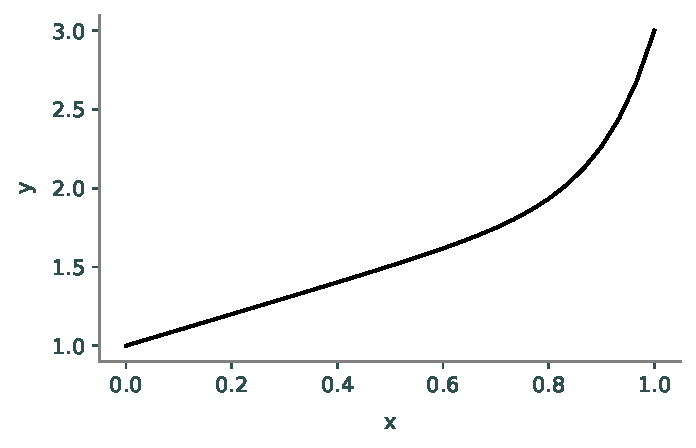
\includegraphics[width=10cm]{figures/figure2.pdf}
\caption{The solution to Problem \ref{prob:finitedifference2:prob1}.
The solution gets steeper near $x = 1$ as $\epsilon $ gets small.}
\end{figure}


\section*{A heuristic test for convergence}
\begin{figure}[ht]
\centering
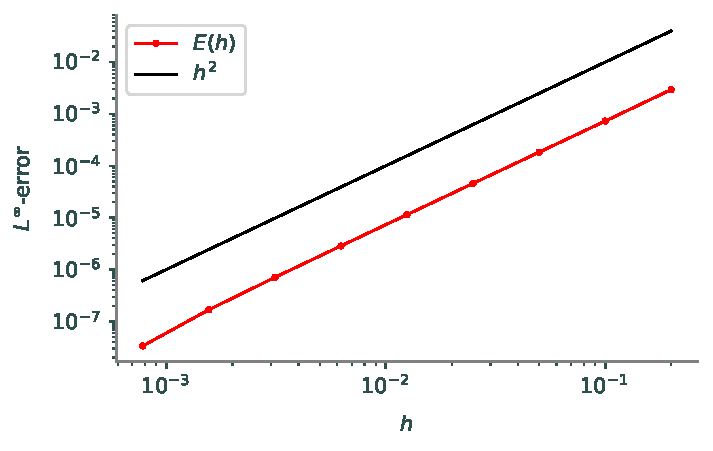
\includegraphics[width=12cm]{figures/example_convergence.pdf}
\caption{Demonstration of second-order convergence for the finite difference approximation \eqref{fd_operator} of the BVP given in \eqref{eqn:singular_perturbed_BVP} with $\epsilon = .5$. } \label{fig:finitedifference2}
\end{figure}

The finite differences used above are second-order approximations of the first and second derivatives of a function.
It seems reasonable to expect that the numerical solution would converge at a rate of about $\mathcal{O}(h^2)$.
How can we check that a numerical approximation is reasonable?

Suppose a finite difference method is $\mathcal{O}(h^p)$ accurate.
This means that the error $E(h) \approx Ch^p$ for some constant $C$ as $h \to 0$ (in other words, for $h>0$ small enough).

So compute the approximation $y_k$ for each stepsize $h_k$, $h_1 > h_2> \ldots>h_m$.
$y_m$ should be the most accurate approximation, and will be thought of as the true solution.
Then the error of the approximation for
stepsize $h_k, k < m,$ is
\begin{align*}
	E(h_k) &= \max( \abs{ y_k - y_m}) \approx C h_k^p ,\\
	\log(E(h_k)) &= \log(C) + p \log(h_k).
\end{align*}

Thus on a log-log plot of $E(h)$ vs. $h$, these values should be on a straight line with slope $p$ when $h$ is small enough to start getting convergence.
We should note that demonstrating second-order convergence does NOT imply that the numerical approximation is converging to the correct solution.


\begin{problem}
Implement a function \li{singular_bvp} to compute the finite difference solution to \eqref{eqn:singular_perturbed_BVP}.
Using $n = 5 \times 2^0,5 \times 2^1, \dots ,5 \times 2^9$ subintervals, compute 10 approximate solutions. 
Use these to visualize the $\mathcal{O}(h^2)$ convergence of the finite difference method from Problem \ref{prob:finitedifference2:prob1} by producing a loglog plot of error against subinterval count; this will be similar to Figure \ref{fig:finitedifference2}, except with $\epsilon=0.1$.
Also plot $h^2$ on the same plot, as in Figure \ref{fig:finitedifference2}.
Remember to use sparse matrices.

To produce the plot, treat the approximation with $n = 5 \times 2^9$ subintervals as the ``true solution,'' and measure the error for the other approximations against it.
Note that, since the ratios of numbers of subintervals between approximations are multiples of 2, we can compute the $L_{\infty}$ error for the $n=5 \times 2^j$ approximation by using the \li{step} argument in the array slicing syntax:
\begin{lstlisting}
# best approximation; the vector has length 5*2^9+1
sol_best = singular_bvp(eps,alpha,beta,f,5*(2**9))

# approximation with 5*(2^j) intervals; the vector has length 5*2^j+1
sol_approx = singular_bvp(eps,alpha,beta,f,5*(2**j))

# approximation error; slicing results in a vector of length 5*2^j+1,
#    which allows it to be compared
error = np.max(np.abs(sol_approx - sol_best[::2**(9-j)]))
\end{lstlisting}
\end{problem}

Consider a similar, but somewhat generalized ODE of the form in (\ref{eqn:singular_perturbed_BVP}),

\begin{align*}
	&{ } a_1(x)y''(x) +a_2(x)y'(x) +a_3(x)y(x) = f(x), \quad x \in (a,b),\\
	&{ } y(a) = \alpha, \quad y(b) = \beta.
\end{align*}
The functional coefficients $a_1, a_2, a_3$ can be treated similarly to constant coefficients, but with each row corresponding to a gridpoint in $x$ (but not including the endpoints).
Applying the finite difference approximations gives the following system of equations:
\begin{align*}
\frac{1}{h^2} & \left( \left(-2a_1(x_1) + h^2a_3(x_1)\right)U_1 + \left(a_1(x_1) + \frac{h}{2}a_2(x_1)\right)U_2  \right) \\
&\hspace{7cm} = f(x_1) - \alpha \left(\frac{a_1(x_1)}{h^2}- \frac{a_2(x_1)}{2h}\right) \\
\frac{1}{h^2} & \left( \left(a_1(x_2) - \frac{h}{2}a_2(x_2)\right) U_1 + \left(- 2a_1(x_2) + h^2a_3(x_2)\right)U_2  + \left(a_1(x_2) + \frac{h}{2}a_2(x_2) \right)U_3 \right) \\
&\hspace{7cm}= f(x_2)
\\
&\hspace{7cm}~~\vdots
\\
\frac{1}{h^2}& \left( \left(a_1(x_k) - \frac{h}{2}a_2(x_k)\right) U_{k-1} + \left(- 2a_1(x_k) + h^2a_3(x_k)\right)U_k + \left(a_1(x_k) + \frac{h}{2}a_2(x_k) \right)U_{k+1} \right) \\
&\hspace{7cm}= f(x_k) \\
\end{align*}\begin{align*}
&\hspace{7cm}~~\vdots \\
\frac{1}{h^2}& \left( \left(a_1(x_{n-1}) - \frac{h}{2}a_2(x_{n-1})\right) U_{n-2} + \left(- 2a_1(x_{n-1}) + h^2 a_3(x_{n-1})\right)U_{n-1} \right) \\
&\hspace{7cm}= f(x_{n-1}) 
- \beta\left(
\frac{a_1(x_{n-1})}{h^2}+ \frac{a_2(x_{n-1})}{2h}
\right)
\end{align*}

This can (and should) be put into matrix form to be solved.
It was not done here because it requires more page space than is available.

\begin{problem}
Extend your finite difference code to the case of a general second-order linear BVP with boundary conditions:
\begin{align*}
	&{ } a_1(x)y''(x) +a_2(x)y'(x)+ a_3(x) y(x) = f(x), \quad x \in (a,b),\\
	&{ } y(a) = \alpha, \quad y(b) = \beta.
\end{align*}
Use your code to solve the boundary value problem
\begin{align*}
	\epsilon y'' - 4(\pi - x^2)y = \cos x, \\
	y(0) = 0, \quad y(\pi/2) = 1,
\end{align*}
for $\epsilon = 0.1$ on a grid with $n=30$ subintervals.
\label{prob:finitedifference2:prob3}
Be sure to modify the finite difference operator $D_h$ in \eqref{fd_operator} correctly.
Remember to use sparse matrices.

\end{problem}



\begin{figure}[h]
\centering
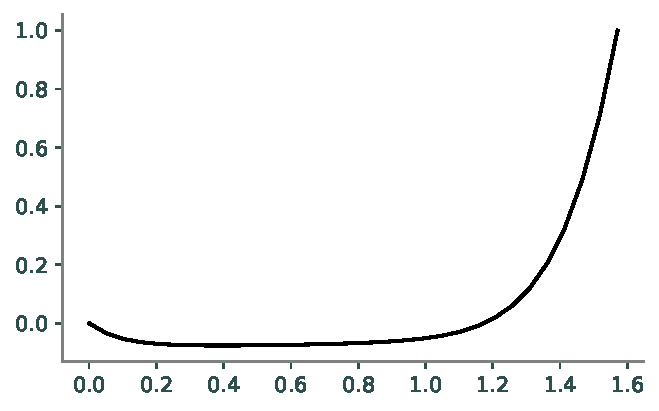
\includegraphics[width=10cm]{figures/figure3.pdf}
\caption{The solution to Problem \ref{prob:finitedifference2:prob3}.
% The solution gets steeper near $x = 1$ as $\epsilon $ gets small.
}
\end{figure}


The next few problems will help you test your finite difference code.

\begin{problem}
Numerically solve the boundary value problem
\begin{align*}
	\epsilon y''(x) + xy'(x) = -\epsilon \pi^2 \cos(\pi x) - \pi x \sin(\pi x), \\
	y(-1) = -2, \quad y(1) = 0,
\end{align*}
for $\epsilon = 0.1, 0.01,$ and $0.001$.
Use a grid with $n=150$ subintervals.
Plot your solutions.
\label{prob:finitedifference2:prob4}
\end{problem}

\begin{problem}
Numerically solve the boundary value problem
\begin{align*}
	(\epsilon +x^2)y''(x) + 4xy'(x) + 2y(x) = 0, \\
	y(-1) = 1/(1+\epsilon), \quad y(1) = 1/(1+\epsilon),
\end{align*}
for $\epsilon = 0.05, 0.02$.
Use a grid with $n=150$ subintervals.
Plot your solutions.
\label{prob:finitedifference2:prob5}
\end{problem}

\begin{figure}[h]
\centering
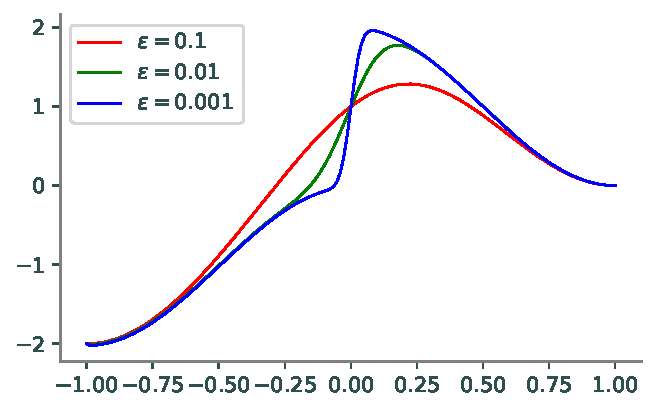
\includegraphics[width=11cm]{figures/figure4.pdf}
\caption{The solution to Problem \ref{prob:finitedifference2:prob4}.
}
\end{figure}

\begin{figure}
\centering
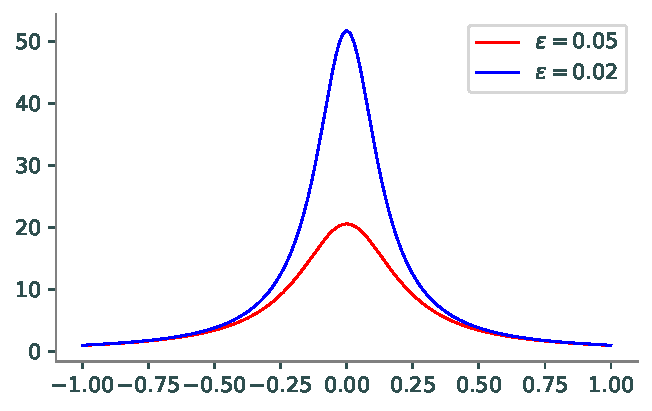
\includegraphics[width=11cm]{figures/figure5.pdf}
\caption{The solution to Problem \ref{prob:finitedifference2:prob5}.
}
\end{figure}
